\chapter{Stand van zaken}
\label{ch:stand-van-zaken}

% Tip: Begin elk hoofdstuk met een paragraaf inleiding die beschrijft hoe
% dit hoofdstuk past binnen het geheel van de bachelorproef. Geef in het
% bijzonder aan wat de link is met het vorige en volgende hoofdstuk.

% Pas na deze inleidende paragraaf komt de eerste sectiehoofding.
\section{Be-Mobile}
\label{sec:Be-Mobile}
Er zijn een groot aantal microservices door Be-Mobile ontwikkeld in Go om verkeersevents op te halen, te verwerken, en door te sturen. Een file met events wordt binnengehaald via een repository en naar JSON omgezet om naar Kafka te sturen. Kafka is een message broker. Dit is in essentie een message queue waarin volgorde kan gegarandeerd worden. Kafka zelf bestaat uit producer- en consumertopics, waar data respectievelijk naar geschreven en uit opgehaald wordt. Daarna worden de messages opgehaald uit kafka en wordt elk individueel event verrijkt met locatie, omschrijving, en andere zaken. Elke stap in de chain haalt de events op van Kafka, communiceert met API's om deze te verrijken en stuurt ze daarna terug naar een andere Kafka topic.

Om deze microservice architectuur te runnen wordt gebruik gemaakt van Kubernetes en Docker. Deze twee technologiën zijn enorm belangrijk in het hele verhaal en worden nog verder uitgelegd in 2.4 Kubernetes, en 2.5 Docker. In het kort is Kubernetes een cluster van nodes die gebruik maken van gecontaineriseerde events. Deze containers worden mogelijk gemaakt dankzij Docker. Elk event wordt niet door dezelfde chain van services gestuurd, er zijn meerdere mogelijke chains die doorlopen kunnen worden. De Kubernetes cluster bevat alle mogelijke chains waar elke service zijn eigen console heeft. Op het moment van het schrijven van dit werk is de enige logging die aanwezig is bij Be-Mobile de verzameling van console logs van Kubernetes. Om te debuggen moet er voortdurend gewisseld worden van console om het probleem te localiseren. Er is nog geen mogelijkheid tot filteren, gericht zoeken, of log metrics \autocite{jens2019}.

\section{Golang}
\label{sec:Golang}
De taal die steeds meer gebruikt wordt in microservice architecturen is Go \Autocite{Sabic2018}. De redenen hiervoor worden mooi beschreven door IT Marketplace. Deze stelt dat microservices het best geschreven worden in Go omwille van:
\begin{enumerate}
    \item “Go is snel en relatief snel te leren” \autocite{ITMarketplace2016};
    \item “Een Go programma in de vorm van een enkel binair bestand is gemakkelijk te deployen” \autocite{ITMarketplace2016};
    \item “Een Go programma is gemakkelijk te omwikkelen in een container” \autocite{ITMarketplace2016};
\end{enumerate}
Golang is een expressieve, beknopte, en efficiënte taal met een nadruk op concurrency en modulariteit \autocite{Golang2012}.

\section{Microservices}
\label{sec:microservices}

Een microservice architectuur bestaat uit vele kleine services die elk hun eigen verantwoordelijkheid hebben, maar samen dezelfde functionaliteit bevatten als een monolithische architectuur (zie figuur 2.1). Het grote verschil met deze tweede is dus de structuur waarop deze is gebaseerd. Waar een monolithische architectuur bestaat uit één groot stuk software vol samenhangende componenten, bevat een microservice architectuur tientallen of zelfs honderden kleine services die met elkaar verbonden zijn in een chain. Events worden van de ene service naar de andere doorgestuurd, vaak door middel van een HTTP requests en message brokers \autocite{Casey2017}. 

\begin{figure}[ht]
    \centering
    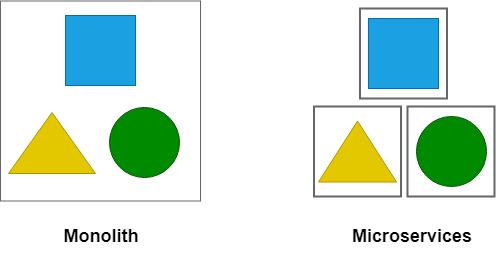
\includegraphics[scale=0.6]{img/monolith-vs-micro}
    \caption[Vergelijking tussen een monolith en microservices applicatie]{Vergelijking tussen een monolith en microservices applicatie \cite{SourceFuse2018}}
\end{figure}

Een microservice architectuur wordt steeds meer gebruikt in organisaties bij het ontwikkelen van hun applicaties. Dit vooral omwille van voordelen zoals simpliciteit en flexibiliteit. Een ander voordeel aan het implementeren van microservices is het gemak waarmee fouten kunnen opgespoord en behandeld worden. Wanneer een service fouten produceert, zal deze sneller te vinden zijn. Aangezien een enkele service vaak slechts een klein stuk software betreft, zal het probleem snel opgelost kunnen worden. Er is dus sprake van een verhoogd overzicht in de structuur van een applicatie. De schaalbaarheid en het onderhoudsgemak zijn nog twee belangrijke zaken om te vermelden. Er is ook een negatief aspect aan microservices verbonden, namelijk een enorm planning aspect bij de implementatie van deze structuur. Indien op een foute manier toegepast, kan het leiden tot een gedistribueerde monolithische structuur, wat het slechtste van de twee werelden combineert \autocite{Carey2018}. 

Logging is een enorm belangrijk aspect van een microservice architectuur. Om een applicatie met microservices te kunnen debuggen moet er een gecentraliseerd logging platform aanwezig zijn. Hoe groter de applicatie, hoe moeilijker om het overzicht van al deze services te bewaren. Elke service heeft een aparte console waarnaartoe gelogd wordt. Dit maakt het moeilijk om alles te doorzoeken in geval van bugs \autocite{SourceFuse2018}. 

Be-Mobile maakt gebruik van een microservice architectuur om hun producten te ontwikkelen. Elk verkeersevent dat binnenkomt, wordt van de ene microservice naar de andere doorgegeven en steeds verder verwerkt. Zo wordt een chain gecreëerd. Er zijn meerdere chains die doorlopen kunnen worden. Dit hangt af van het soort event dat heeft plaatsgevonden. Een belangrijk punt bij het implementeren van een gecentraliseerd logging platform voor Be-Mobile is dus het visualiseren van de chain die gevolgd werd door een bepaald event door middel van tracing \autocite{jens2019}.

\section{Kubernetes}
\label{sec:kubernetes}

\subsection{Wat is Kubernetes?}
De basis van Kubernetes is dat het een open-source systeem is voor het beheren van applicaties die in een container (zie 2.5 Docker) geplaatsd zijn. Containers zijn omhulsels voor services. Alles wat nodig is om de service te kunnen runnen, wordt voorzien door de container. Kubernetes draait als een samenhangende cluster (zie figuur 2.2) zodat men  componenten en services doorheen verschillende infrastructuren kan beheren. De manier waarop applicaties gehost worden hangt af van de manier waarop Kubernetes geconfigureerd is. Het is mogelijk om een applicatie te runnen als een DaemonSet, waardoor er in elke node een instantie van de applicatie gerund wordt. Ook zorgt deze configuratie er voor dat er automatisch een nieuwe instantie van de applicatie gecreëerd wordt bij het aanmaken van een nieuwe node. Dit is slechts een voorbeeld van de mogelijkheden van Kubernetes. De optimale configuraties van de onderzochte logging solutions komen later aan bod in de bijlagen van dit werk \autocite{ellingwood2018}.

\begin{figure}[ht]
    \centering
    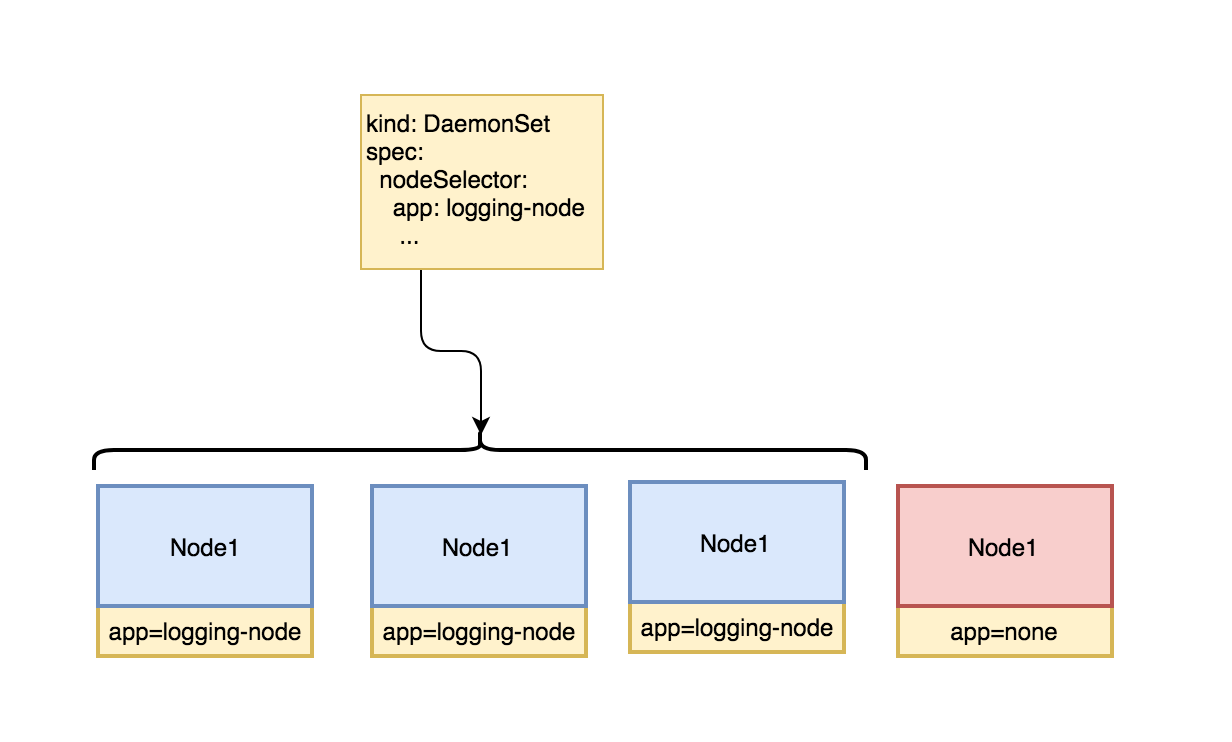
\includegraphics[scale=0.4]{img/kubernetes_daemonset}
    \caption[Kubernetes DaemonSet voorbeeld]{Kubernetes Daemonset voorbeeld \cite{techstories2017}}
\end{figure}

\subsection{Architectuur}
Kubernetes bestaat uit een master-minion architectuur (zie figuur 2.3) waar een master server het brein van de cluster voorstelt. Deze is een gateway om verschillende API's bloot te stellen aan de gebruikers. Verder is de master ook verantwoordelijk voor het controleren van de gezondheid van de cluster, scheduling van alle taken, en de communicatie tussen alle componenten \autocite{ellingwood2018}.

De `minions' worden nodes genoemd en zijn de servers waarop een of meerdere containers gerund worden. De nodes krijgen instucties van de master over wat er moet gebeuren met verschillende containers. Het creëren van nieuwe containers, het vernietigen van oude containers, en het forwarden van data zijn enkele van de taken van de nodes \autocite{ellingwood2018}.

Een node bestaat uit een of meerdere pods (zie figuur 2.3). Elke pod is een groep van een of meerdere containers die gedeployed zijn. Deze pods zijn er om nog verder onderscheid te kunnen maken in de configuratie. Elke pod heeft een eigen IP adres binnen de cluster en elke container in een pod deelt een IP adres, hostnaam, en andere zaken \autocite{learnitguide2018}.

Om een cluster op te starten wordt gebruik gemaakt van configuratie files in de vorm van YAML files. YAML staat voor `YAML Ain't Markup Language` en wordt gebruikt om configuratie mee te maken \autocite{grav}) Hierin wordt de gewenste structuur beschreven. De master server leest deze configuraties en delegeert de opdrachten aan zijn nodes om de gewenste structuur te bereiken \autocite{ellingwood2018}.

Er is ook mogelijkheid tot lokaal testen. Hiervoor wordt Minikube gebruikt. Minikube maakt een lokale cluster aan met één node waarin een aantal pods aangemaakt kunnen worden. Op deze manier is het mogelijk configuraties te testen voordat deze gebruikt worden in productie \autocite{ellingwood2018}.

\begin{figure}[ht]
    \centering
   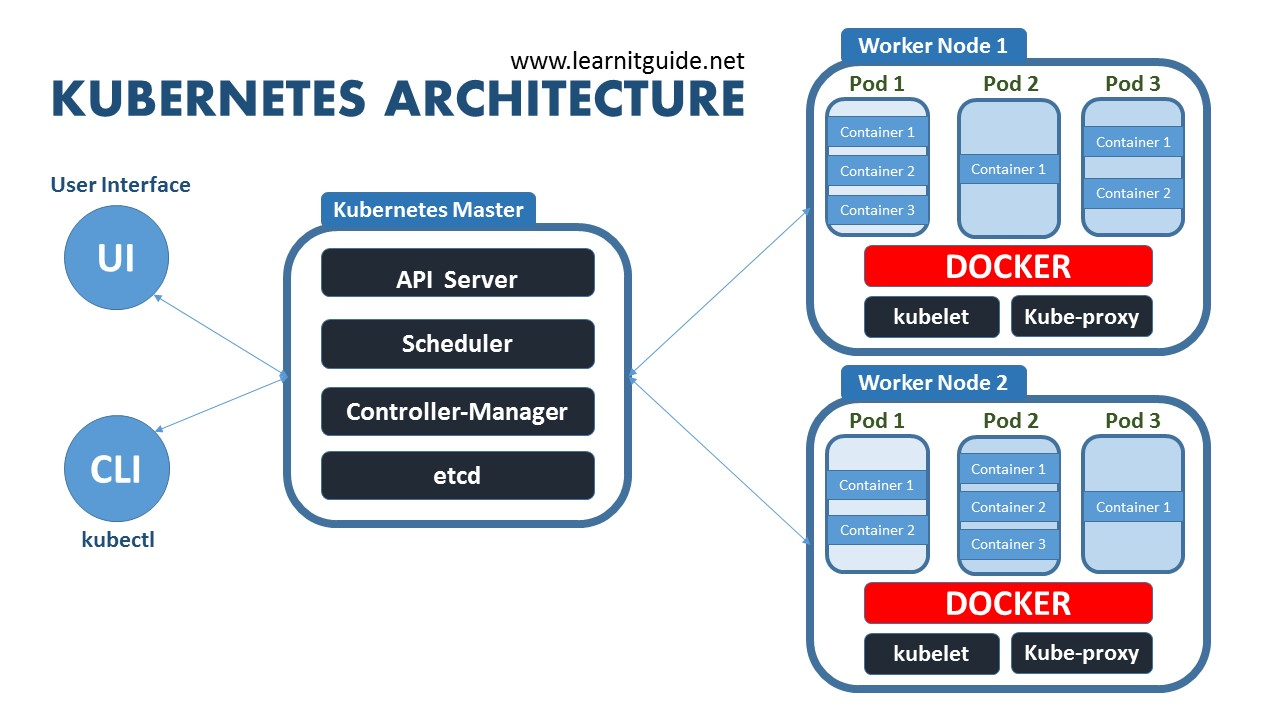
\includegraphics[scale=0.4]{img/kubernetes_architecture_explained}
    \caption[Kubernetes Architecture]{Kubernetes Architecture \cite{learnitguide2018}}
\end{figure}

\section{Docker}
\label{sec:docker}

\subsection{Situatie voor Docker}
Voor de komst van Docker was de manier waarop software uitgevoerd werd volledig anders. Software laat het niet steeds toe om uitgevoerd te worden in dezelfde omgeving als een ander soort software. Maar hoe slaagde men er in om toch alle programma's werkende te krijgen? Ze maakten gebruik van virtual machines. Deze lieten toe om verscheidene programma's simultaan uit te voeren op dezelfde hardware. Hoewel virtuele machines een oplossing boden voor het probleem, was de kost hoog. Virtuele machines zijn zware software die elk enkele gigabytes in grootte zijn.Verder bracht deze oplossing andere problemen met zich mee  zoals software updates, continuous delivery, en continuous integration \autocite{yegulalp2018}.

\subsection{De oplossing}
Docker containers zijn de oplossing voor dit probleem. Ze zijn licht, draagbaar, en flexibel. De manier waarop ze werken is simpel (zie figuur 2.4). Elk programma of stuk software wordt omhuld in een container die afzonderlijk draaiende wordt gehouden zoals een virtuele machine. Kortom wil dit zeggen dat alles geïsoleerd wordt en er dus geen problemen ontstaan met componenten die niet samen kunnen uitgevoerd worden. Zoals reeds besproken maakt Kubernetes uitstekend gebruik van containers. Het brengt deze met elkaar in contact of houdt ze net gescheiden. Zo kunnen containers die afhangen van elkaar, aan elkaar vastgehaakt worden in een pod. Een andere functionaliteit van Docker container is de herbruikbaarheid. Eens een container aangemaakt is kan deze via Kubernetes meerdere malen herbruikt worden of simultaan uitgevoerd worden \autocite{yegulalp2018}.

\begin{figure}[ht]
    \centering
    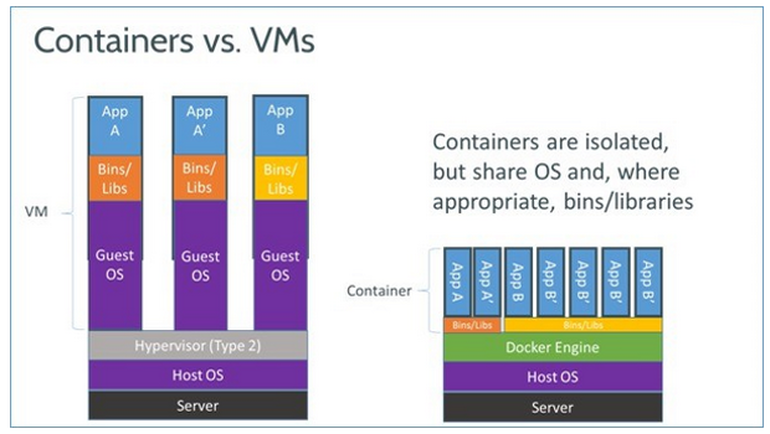
\includegraphics[scale=0.6]{img/docker-vm-vergelijking}
    \caption[Vergelijking tussen VM's en Docker containers]{Vergelijking tussen VM's en Docker containers \cite{vaughan2018}}
\end{figure}

\section{Logs, traces, en metrics}
\label{sec:log}

\subsection{Wat is een log?}

Een log is de documentatie van events die zich voordoen. De meeste systemen en softwareapplicaties bevatten automatische log generatie. De logs worden dan opgeslagen in een file waar ze bijgehouden worden om later geëvalueerd te worden. Men kan ook opteren om bij het schrijven van een eigen applicatie zelf logging te voorzien om de eigen applicatie beter te kunnen opvolgen en te debuggen. De keuze ligt bij de developer om deze logs dan op te slaan in een file. Standaard worden logs getoond in de console met een timestamp, bericht, en een log niveau \autocite{Techopedia}.

\subsection{Belang van logging}

Logging is een belangrijk aspect van software development. Maar wat is nu het belang van logging? De tijd die een developper investeert in het correct loggen van de belangrijke informatie in een applicatie is hopelijk toch geen verspilde tijd? 

Ten eerste is er het belang van duidelijkheid in een applicatie. Logs zorgen er voor dat er precies kan gezien worden wat er gaande is in een applicatie. Bij het debuggen zijn logs van onschatbare waarde om na te gaan wat er fout is gegaan \autocite{logdna2018}.

Ten tweede hebben logs belang voor het hele bedrijf. Wanneer er sprake is van een bedrijf met verschillende teams die elk verantwoordelijk zijn voor hun eigen deel van een applicatie, zullen er restricties te vinden zijn in de rechten van elk team. Een developper hoort geen rechten te hebben op repositories waar hij zelf niet mee in contact komt. Bij het debuggen van een probleem kan een developper de logs van software waar hij zelf geen rechten op heeft toch bekijken. Zonder logs zouden er rechten toegekend moeten worden om de code te bekijken op zoek naar het probleem \autocite{czanik2013}.

\subsection{Golang logging frameworks}

Bij Be-Mobile wordt Golang gebruikt om de backend van hun microservices op te bouwen. Deze relatief nieuwe taal heeft reeds enkele ondersteunde opties op vlak van logging frameworks. De twee meest gebruikte zijn Glog en Logrus \autocite{Dietrich2018}. In dit onderzoek zal enkel Logrus ter sprake komen omdat deze het meest actief ondersteund wordt en omdat Logrus het gekozen logging framework is van Be-Mobile \autocite{jens2019}.

Glog:
\begin{itemize}
    \item Uitgebracht door Google;
    \item Simpele stijl, gebaseerd op die van Golang zelf \autocite{Dietrich2018};
    \item Laatste commit 25 januari 2016 \autocite{Glog2013};
\end{itemize}

Logrus:
\begin{itemize}
    \item Community driven;
    \item Goede ondersteuning;
    \item Laatste commit 3 maart 2019 \autocite{sirupsen2014};
\end{itemize}

\subsection{Logrus}
“Logrus is een gestructureerde logger voor Go, volledig API compatibel met de standaard library logger” (sirupsen, s.d.). Logrus is een uitbreiding op de standaard library logger. Het biedt een wijd gamma aan functionaliteit bij het loggen van events. De verschillende levels waarin gelogd kan worden zijn: Trace, Debug, Info, Warning, Error, Panic, en Fatal. Deze levels zorgen voor een duidelijke weergave van het gelogde event. Hiermee kan de gebruiker, indien deze gebruik maakt van een log collector, filteren op level en zo vlotter de verschillende events doorlopen tijdens het debuggen. Verder kunnen ook nog andere fields toegevoegd worden die de gebruiker extra mogelijkheden biedt tijdens het filteren. Ten slotte kunnen de logs zowel de console als een wijd gamma andere keuzes als output gebruiken. Logrus kan gebruik maken van hooks om de data door te sturen naar message brokers zoals redis en kafka, alsook naar een file die lokaal opgeslagen kan worden. Hooks zijn zoals de term al doet vermoeden inhakingen op logrus. Hiermee kan er vooraleer de logs in de output verschijnen nog iets met gedaan worden \autocite{sirupsen2014}.

\subsection{Tracing}

Naast logs is er nog een tweede soort data die belangrijk is in microservices, trace data. De bedoeling van dit soort data is het achterhalen van de volledige chain die doorlopen wordt door een enkel event. Doorheen de chain kan dan gekeken worden hoelang elke microservice gewerkt heeft of hoelang een bepaalde API-call heeft geduurd (zie figuur 2.5). Deze data kan daarna gebruikt worden om metrics mee te maken, bv. De gemiddelde duur van een API-call. Zo kunnen uitschieters onderzocht worden om tot de kern van een probleem te komen \autocite{Rouse2018}.

OpenTracing is een specificatie welke gebruikt wordt door de grootste Tracers. Omdat OpenTracing vendor-neutral is kan men dus kiezen welke Tracer men uiteindelijk wil gebruiken bij het verzamelen van traces (Rouse, 2018). De meest gebruikte Tracers voor Go zijn Zipkin en Jaeger \autocite{Sabic2018}.

\begin{figure}[ht]
    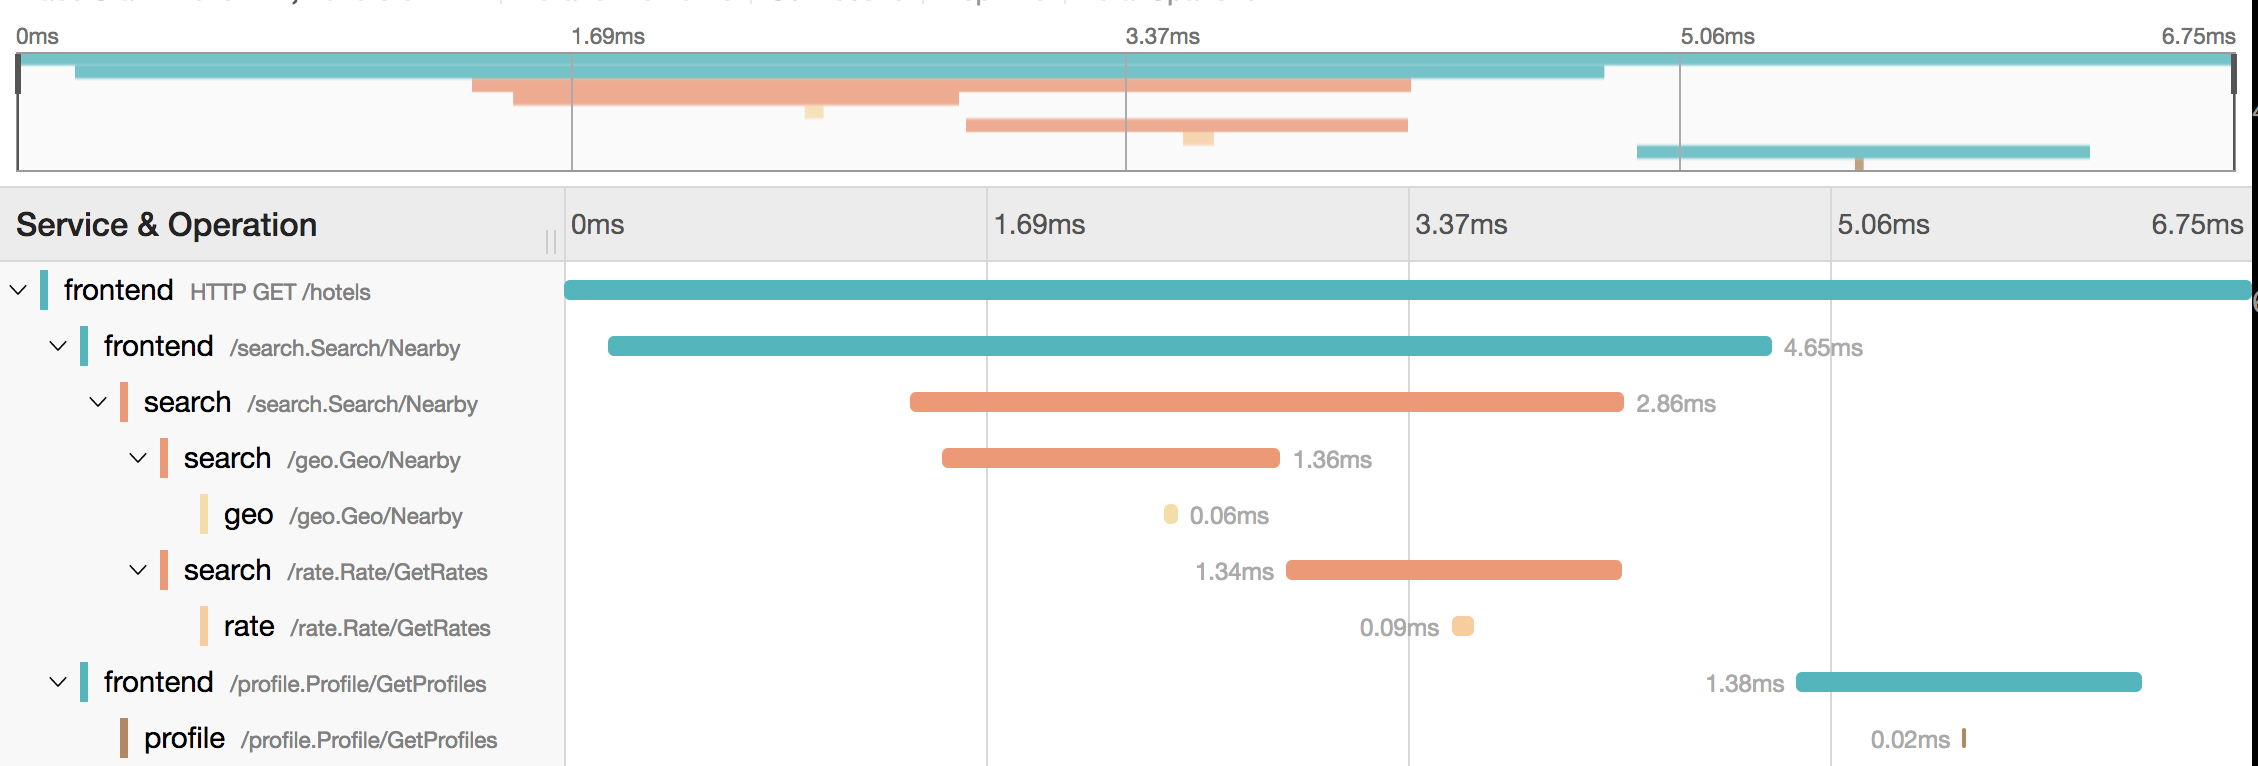
\includegraphics[scale=0.4]{img/tracing_voorbeeld}
    \caption[Voorbeeld van tracing in Jaeger]{Voorbeeld van tracing in Jaeger \cite{harlow2015}}
\end{figure}

\subsection{Metrics}

De derde en laatste soort data die gebruikt wordt om een applicatie te monitoren is metrics. Deze houden de systeembeheerders op de hoogte van de status van de applicatie. Dit werk maakt een vergelijkende studie tussen de meest populaire logging solutions, dus buiten deze korte introductie zal er niet verder ingegaan worden op metrics. Metrics maken het mogelijk om in een oogopslag de algemene gezondheid van een applicatie te zien (zie figuur 2.6). Er wordt gebruik gemaakt van grafieken en statistieken om dit weer te geven. Het verschil met tracing is dat metrics de volledige situatie van een applicatie omvatten en tracing een detail observatie is van bepaalde events of services in de applicatie \autocite{reichert2018}.
\\
\begin{figure}[ht]
    \centering
    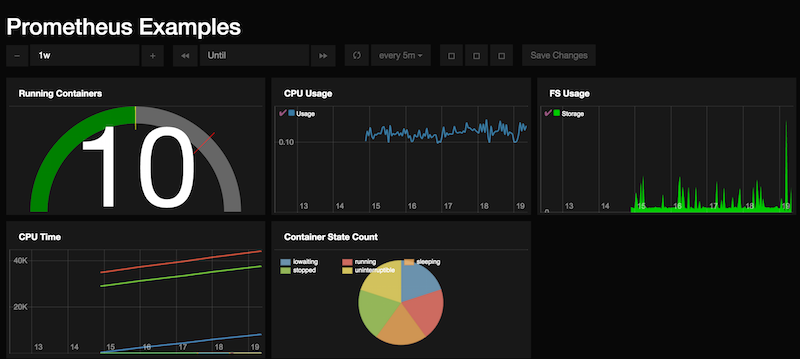
\includegraphics[scale=0.8]{img/prometheus_example}
    \caption[Voorbeeld van metrics in Prometheus]{Voorbeeld van metrics in Prometheus \cite{christner2015}}
\end{figure}

\section{Logging solutions}
\label{sec:logging-solutions}

\subsection{Wat is een logging solution en hoe werkt het?}
Voor er meer in detail gegaan wordt over de logging solutions die getest werden in dit werk, zal er een definitie beschreven worden wat beschouwd wordt als een logging solution.
Een logging solution is een tool of een combinatie van tools die toelaat om efficiënt aan log management te doen. Het hele proces van logging doorloopt verschillende stappen (figuur 2.7) \autocite{logdna2018}.

\begin{figure}[ht]
    \centering
    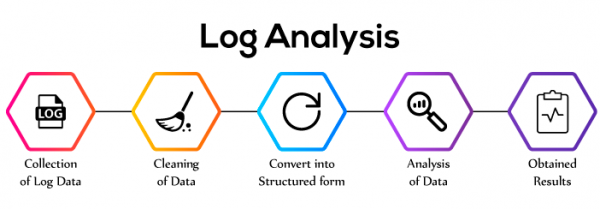
\includegraphics[scale=0.6]{img/log_proces}
    \caption[Het logging proces]{Het logging proces \cite{nastel}}
\end{figure}

\begin{enumerate}
    \item Data collectie: Ingestion en log aggregation. Een eerste stap hierbij is data die verzameld wordt vanuit verschillende bronnen. Deze bronnen kunnen de console logs zijn, de opgeslagen log files, syslog, etc. De verantwoordelijk voor dit proces is een collector. De tweede stap is het correct formateren van de verzamelde logs. Zonder deze stap zou de data niet uniform genoeg zijn om in een latere fase de analyse hierop uit te voeren \autocite{logdna2018}. 
    \item Filtering en analyse: De volgende schakel in het verhaal is de analyse. Eens de logs allemaal hetzelfde formaat hebben, kan er gefilterd worden. Dit kan op verschillende manieren gebeuren. Er kan gefilterd worden op tijd, log level (zie 2.6.4 Logrus), extra toegevoegde tags, service waar de log plaatsvond, en nog veel meer. De analyse gebeurt op basis van grafieken en statistieken. Er is mogelijkheid om bepaalde statistieken bij te houden om gemakkelijk het overzicht te bewaren over situaties die zich kunnen voordoen  \autocite{logdna2018}.
    \item Reporting. Nadat de analyse afgerond is en alle grafieken en statistieken aangemaakt zijn, kan er reporting ingesteld worden voor deze. Er kunnen alarmen aangemaakt worden die op verschillende manieren de verantwoordelijke personen op de hoogte stellen dat een bepaalde situatie zich heeft voorgedaan. Bijvoorbeeld wanneer een service een bovengemiddeld aantal error logs produceert op korte termijn  \autocite{logdna2018}.
    \item Opslag. Hierbij worden logs opgeslagen voor een bepaalde duur zodat deze beschikbaar blijven  \autocite{logdna2018}.
\end{enumerate}

\subsection{Belangrijke punten in een logging solution}

Wat is er belangrijk bij het zoeken naar een logging solution? Waar moet rekening mee gehouden worden in een beslissing?

\begin{enumerate}
    \item  Schaalbaarheid is van enorm belang in de groeiende sector van IT. Een bedrijf dat snel groeit kan zich niet veroorloven steeds opnieuw de hele structuur aan te passen om deze te laten meegroeien. Een goede logging solution kan automatisch of met zo weinig mogelijk werk meegroeien met het bedrijf \autocite{logdna2018}. Een voorbeeld hierin is Be-Mobile (zie 2.1 Be-Mobile) \autocite{jens2019}. 
    \item Overhead. Dit is de impact van de gekozen oplossing op het systeem. Zware oplossingen kunnen de applicatie vertraging en minder performant maken \autocite{gifford2015}.
    \item Installatie \autocite{logdna2018}.
    \item Gebruiksgemak. Alle developpers in het bedrijf moeten dezelfde tool kunnen gebruiken \autocite{logdna2018}.
    \item Snelheid waarmee logs getoond kunnen worden in de gekozen visualisatie tool \autocite{logdna2018}.
    \item Automatische parsing van de logs bij het innemen van de logs \autocite{logdna2018}.
\end{enumerate}

\subsection{ELK}
\label{subsec:ELK}
ELK is een acronym voor Elasticsearch, Logstash, Kibana. Dit zijn de drie componenten die een ELK stack bevat. Vaak wordt bovenop deze componenten ook gebruik gemaakt van Beats. Dit is een lichtgewicht data collector die handig kan zijn bij Kubernetes deployments met vele nodes. Bij complexe pipelines zoals Be-Mobile waar een hoge throughput aan data aanwezig is, wordt aangeraden om gebruik te maken van een message broker tussen de data collectie en data processing die voor een betrouwbare volgorde zorgt. Voorbeelden hiervan zijn Kafka, RabbitMQ, Redis (zie figuur 2.8) \autocite{berman2018-12}. 

\begin{figure}[ht]
    \centering
    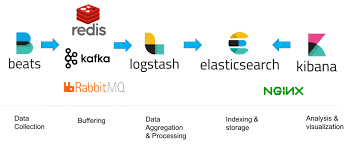
\includegraphics[scale=1]{img/elk-proces}
    \caption[Volledige ELK stack]{Volledige ELK stack \cite{berman2018-12}}
\end{figure}

De werking van ELK gaat als volgt. Logs worden geproduceerd en opgeslagen in files. Beats verzamelt deze en stuurt ze meteen door naar een message broker. Daarna volgt Logstash. Deze haalt de logs op van de message broker en verwerkt deze. De logs worden hier gefilterd. Er kunnen via grok nieuwe benamingen gegeven worden aan delen van de log lijn. Ook kunnen dingen zoals datum, IP-adres, en dergelijke toegevoegd worden. Uiteindelijk worden de logs doorgestuurd naar Elasticsearch waar ze opgeslagen worden. De werking van Logstash wordt volledig bepaald door een config file. De laatste stap is Kibana, dit is de visualitie tool. Kibana gebruikt Elasticsearch als data source om de logs op te halen en toont deze met extra kleur accenten op tags om duidelijkheid te creëren \cite{levy2015,berman2018-12}. 

De ELK stack is een goede logging oplossing omdat het een enorm krachtige tool is in combinatie met een gemakkelijk installatie. Naast zijn vele voordelen zijn er ook wat mindere punten aan de ELK stack die genoemd moeten worden. Hoewel de basis installatie vrij simpel uit te voeren is, wordt deze al snel ingewikkelder naargelang de grootte van de cluster waarop deze geïnstalleerd wordt. Er zijn veel factoren waar rekening gehouden mee moet worden en een verkeerde implementatie kan leiden tot inefficiëntie of zelfs crashes op lange termijn. Om deze reden hoort er genoeg aandacht besteed te worden aan resource management bij het opzetten van de ELK stack \autocite{gifford2016}.

\subsection{EFK}
\label{subsec:EFK}

\begin{figure}[ht]
    \centering
    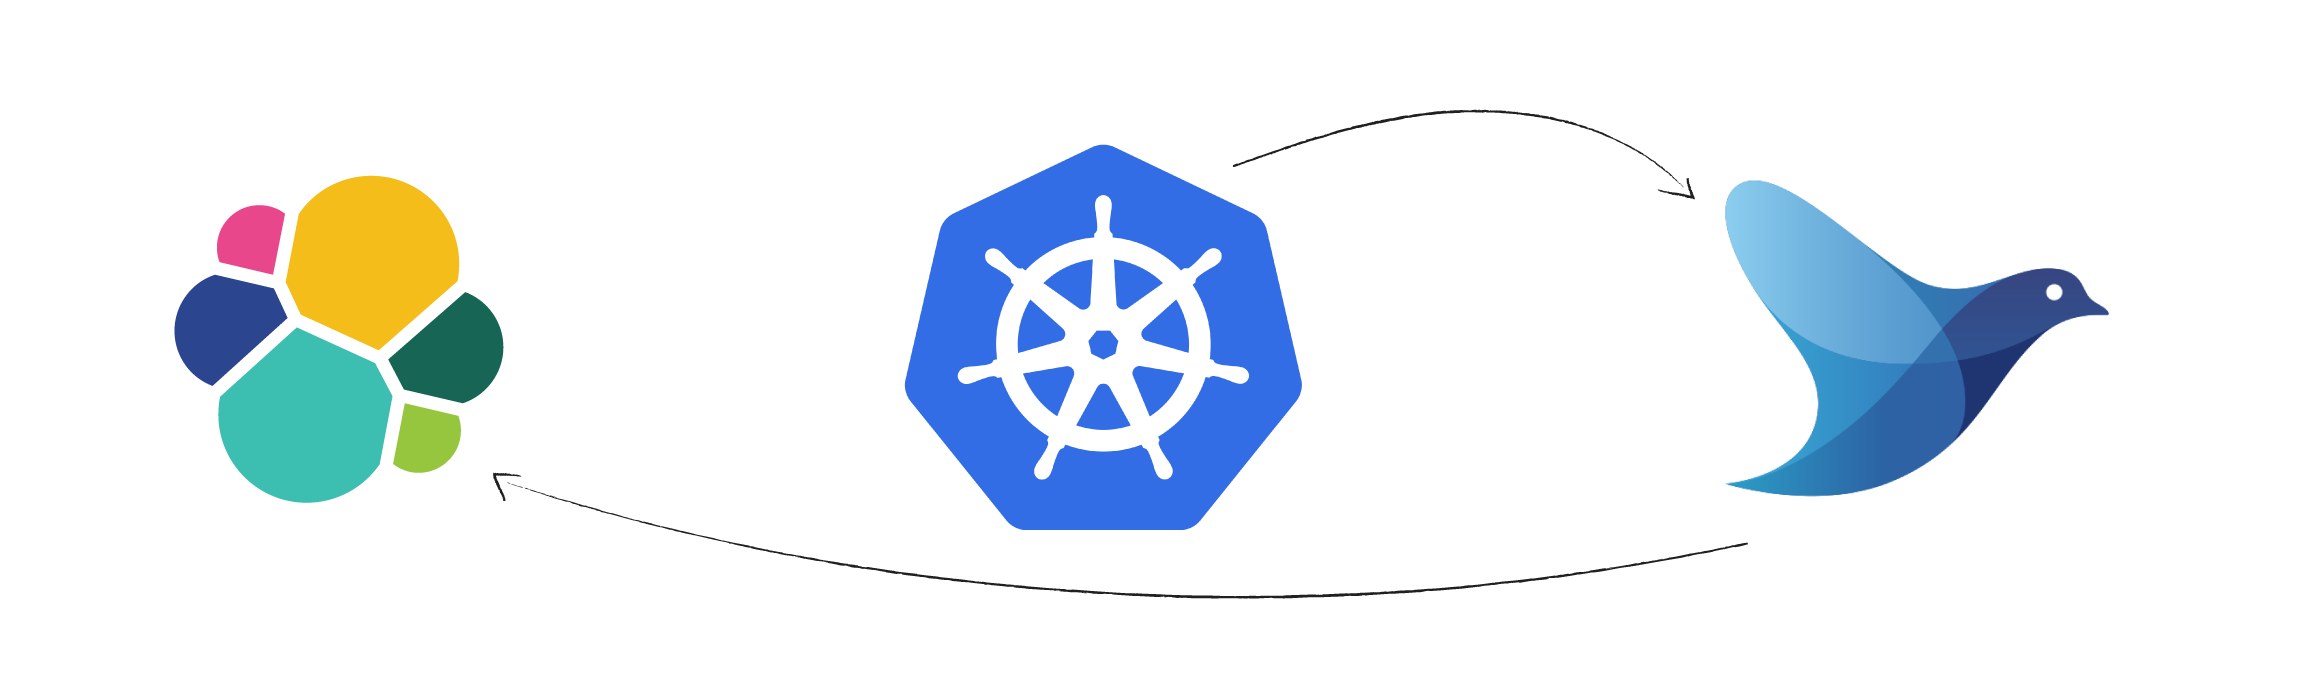
\includegraphics[scale=0.15 ]{img/EFK_logo}
    \caption[EFK stack]{EFK stack \cite{petrausch}}
\end{figure}

Soortgelijk aan ELK, is EFK een acronym voor Elasticsearch, Fluentd, Kibana (zie figuur 2.9). Hierbij wordt op een soortgelijke manier gewerkt als bij ELK maar wordt Logstash vervangen door Fluentd. De redenen hiervoor zullen hieronder verder uitgelegd worden. Wanneer gewerkt wordt met Kubernetes moet de afweging gemaakt worden tussen gebruik van Fluentd en Fluentbit. Deze laatste is een nieuwere, kleinere variant van de eerste. Qua functionaliteit zijn ze beiden bijna evenwaardig met als enige grote verschil het aantal ondersteunde plugins wat veel hoger is bij Fluentd. De grote kracht van Fluentbit is dan weer de grootte ervan. Met slechts 450KB is de voetafdruk van Fluentbit op gedistribueerde omgevingen enorm klein in vergelijking met Fluentd. Fluentbit is dan ook ontwikkeld met gedistribueerde omgevingen als primaire use case \autocite{berman2018-06}.

Deze verschillen tussen Logstash en Fluentd zijn als volgt:
\begin{enumerate}
    \item Taal. Logstash is geschreven in JRuby welke een Java implementatie is van Ruby en dus een Java Runtime vereist. Fluentd daarentegen is geschreven in CRuby, een C implementatie van Ruby en heeft dus minder vereisten qua omgeving.  \autocite{harikumar2018}.
    \item De routing van events. Waar Logstash voor routing zorgt door gebruik te maken van if-then statements, gebruikt Fluentd tags om hetzelfde te doen. Fluentd lijkt daarop iets makkelijk om te configureren \autocite{harikumar2018}.
    \item Plugins. Zoals eerder vermeld heeft Fluentd een enorm grote hoeveelheid plugins met meer dan 350 plugins voor input, output, of verwerking van data. Logstash beschikt ook over een aantal plugins. Het grote verschil zit in de plaats waar deze plugins te vinden zijn. In tegenstelling tot Fluentd is er bij Logstash wel een gecentraliseerde github repository waar alle plugins te vinden zijn \autocite{harikumar2018}.
    \item Message queue. Door gebruik te maken van Fluentd of Fluentbit wordt de nood aan een message broker geëlimineerd. Fluentd heeft namelijk een ingebouwde message queue die alle inkomende messages zelf correct verwerkt. Hierdoor kan Fluentd, in tegenstelling tot Logstash, geïmplementeerd worden in complexe systemen zonder externe message broker \autocite{harikumar2018}. 
    \item Geheugenverbruik. Waar Logstash gemiddeld 120MB aan geheugen gebruikt, zal Fluentd hetzelfde kunnen doen met maar 40MB. Beide blijven aan de hoge kant wanneer men een situatie schetst waar gebruik gemaakt wordt van honderden servers. De ontwikkelaars van beide log verzamelaars hebben een oplossing uitgebracht. Voor Logstash is dit Filebeat met een gemiddeld geheugen gebruik van 1,8MB. Voor Fluentd is dit Fluentbit met een gemiddeld geheugen gebruik van 450KB \autocite{peri2015}.
\end{enumerate}

Om optimaal gebruik te maken van de EFK stack in een gedistribueerde omgeving op een Kubernetes cluster moet gebruik gemaakt worden van zowel Fluentbit als Fluentd. In deze setup bevat elke node in de cluster een Fluentbit pod die de logs van die node verzameld en doorstuurt naar de algemene Fluentd pod op de cluster. Deze fungeert als aggregator en verwerkt de logs om ze daarna door te sturen naar de gekozen output \autocite{berman2018-06}.

\subsection{Graylog}
\label{subsec:graylog}
Graylog is ontstaan in 2009 in een tijd waar logging oplossingen, laat staan open source logging oplossingen quasi onbestaand waren. De marktleider in die tijd had een kostelijke licentie en daarom ontwikkelde de oprichter van Graylog een eigen open source oplossing. Dit wil zeggen dat Graylog vanaf het begin al een logging oplossing hoorde te zijn. Dit in tegenstelling tot ELK op basis van Elasticsearch, welke een full text search engine is. Graylog maakt zelf ook nog steeds gebruik van Elasticsearch als opslagplaats maar dankzij de Graylog server die voor de databank gepositioneerd is wordt het gebruik ervan geoptimaliseerd voor logs \autocite{graylog}.

De ouderdom van de Graylog betekent dat deze niet is geoptimaliseerd voor het gebruik ervan in een gedistribueerde omgeving zoals een Kubernetes cluster. Er is wel reeds documentatie toegevoegd om Graylog werkende te krijgen op een Kubernetes cluster \autocite{lumiq2017}.  

Graylog maakt voornamelijk gebruik van een eigen log format dat geoptimaliseerd is voor Elasticsearch, namelijk GELF. Dit staat voor Graylog Extender Log Format. GELF is ondersteund als output bij verschillende log forwarders \autocite{graylog}. 

\subsection{Grafana Loki}
De meest recente logging solution, nog steeds in alfa ontwikkeling maar wel reeds beschikbaar. Wat meteen duidelijk wordt, is dat Loki ontwikkeld is voor het gebruik in grote, complexe, gedistribueerde omgevingen. Het is ontwikkeld om zoveel mogelijk logs te kunnen opslaan voor zo weinig mogelijk geld. Tot hiertoe zijn alle databanken gebaseerd op volledige indexering bij het opslaan van logs, dit zorgt voor heel wat opslagruimte die noodzakelijk is om alles draaiende te houden. Loki stapt af van indexering en is gebaseerd op Prometheus, een ander product van Grafana dat gebruikt wordt voor de opslag van metrics. De manier waarop Loki logs opslaat, werkt op basis van labels en enkel de metadata wordt geïndexeerd \autocite{oleksii2019}.

\begin{figure}[ht]
    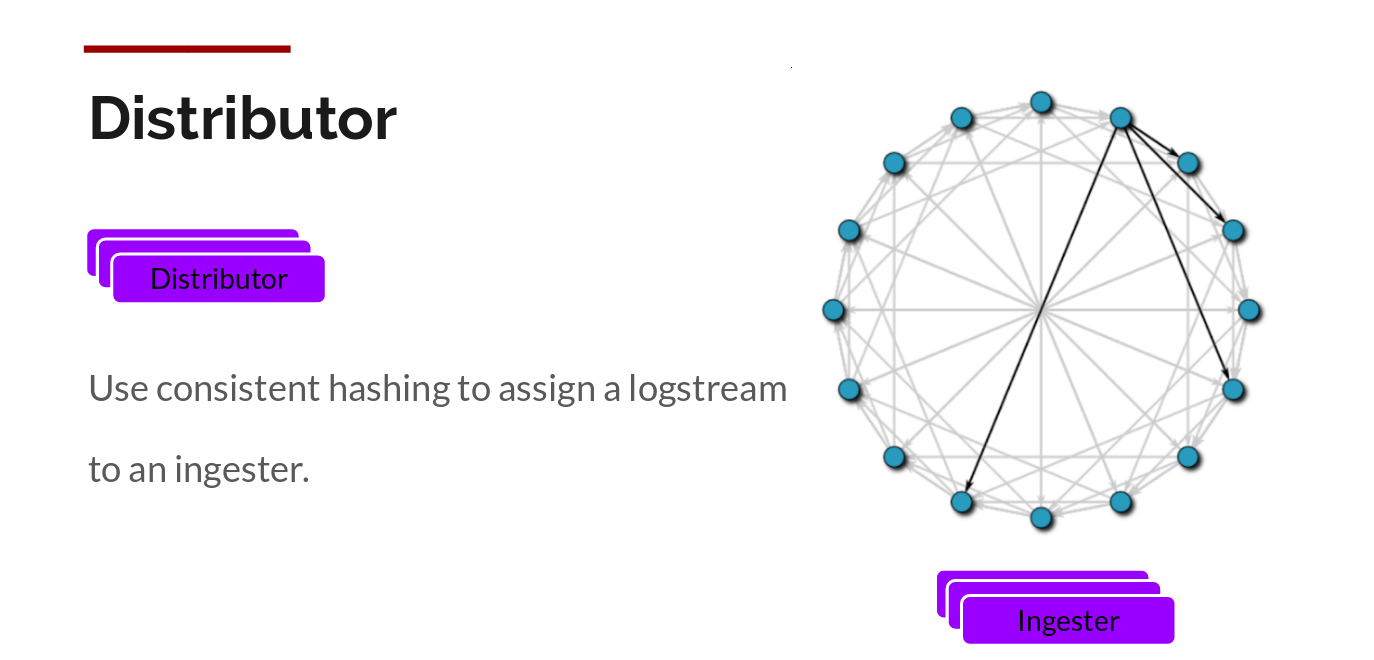
\includegraphics[scale=0.3]{img/loki_distributor}
    \caption[Grafana Loki distributor]{Grafana Loki distributor \cite{loki}}
\end{figure}

\begin{figure}[ht]
    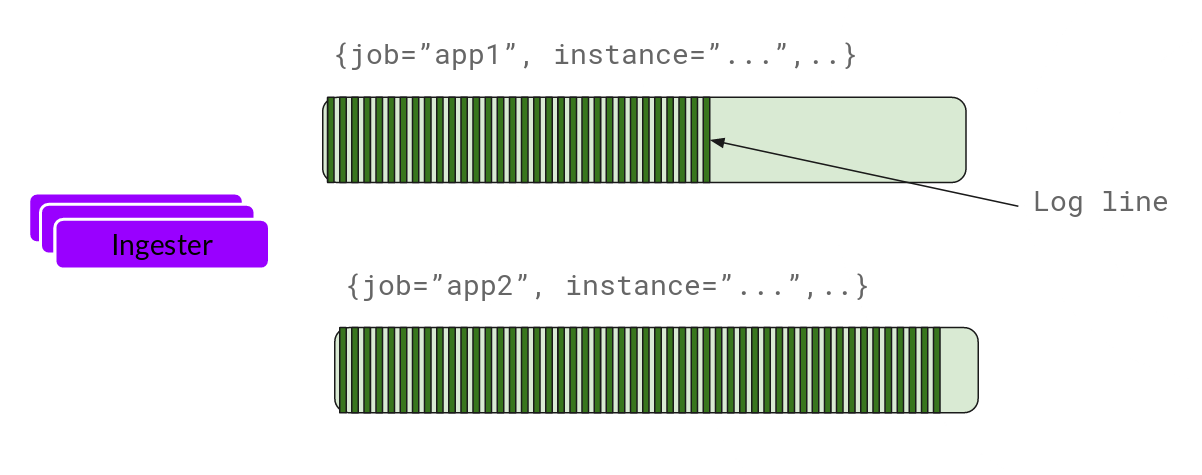
\includegraphics[scale=0.3]{img/loki_ingester}
    \caption[Grafana Loki Ingester]{Grafana Loki Ingester \cite{loki}}
\end{figure}

Een loki 'stack' bestaat uit 3 belangrijke componenten:
\begin{enumerate}
   \item Promtail is verantwoordelijk voor het verzamelen van logs. Het is een scraper die op zoek gaat in alle Kubernetes pods naar log files en deze daarna doorstuurt naar Loki. Promtail wordt geïnitialiseerd op basis van een config file waarin beschreven wordt welke log files doorgestuurd worden, welke genegeerd worden, en welke anders genoemd worden. Soortgelijk aan Fluentbit zal Promtail ook in elke node aanwezig zijn en logs doorsturen naar een algemene loki instantie \autocite{veeramachaneni2018}.
   \item Loki is de datasource van de stack. Het maakt gebruikt van een distributor (zie figuur 2.10) om logs te verspreiden over verschillende ingesters (zie figuur 2.11) vooraleer de logs in een databank terecht komen. De manier waarop Loki logs opslaat is ook anders dan de concurrentie. De ingesters verzamelen soortgelijke logs in chunks. Wanneer een chunck opgevuld is, wordt deze opgeslagen in een Object Storage. Default is dit een lokale Object Storage. De indexen van deze logs worden daarna in een NoSQL database opgeslagen om snel opgehaald te kunnen worden. Deze manier van opslag zorgt voor een snelle ophaling van logs wanneer deze opgevraagd worden in Grafana. Ook zorgt deze manier van opslag voor een grote schaalbaarheid \autocite{veeramachaneni2018}.
   \item Grafana is de frontend die zowel Loki als Prometheus en andere bronnen kan gebruiken als data source. Hier worden de logs gevisualiseerd. Op moment van schrijven van dit werk is er enkel tekstuele filtreerbaarheid beschikbaar op basis van een eigen query taal van Grafana. Ook deze is nog onder constructie en verwacht binnenkort een upgrade. Nummers worden dan ook filtreerbaar met mogelijkheid tot filteren op datum of bepaalde getallen vergelijken \autocite{githubLoki2019, veeramachaneni2018}. 
\end{enumerate}
